\documentclass[11pt,a4paper]{article}
\usepackage[T1]{fontenc}
\usepackage[utf8]{inputenc}
\usepackage{lmodern,microtype}
\usepackage{amsmath,amssymb,amsthm,mathtools,bm}
\usepackage{booktabs,array,tabularx,longtable,multirow}
\usepackage{graphicx,float,caption}
\usepackage{xcolor}
\usepackage[margin=22mm]{geometry}
\usepackage{enumitem,fancyhdr,hyperref,pdflscape}

\definecolor{finblue}{HTML}{1F5A99}
\definecolor{fingreen}{HTML}{19733A}
\definecolor{finorange}{HTML}{C45A00}
\definecolor{finred}{HTML}{A61B1B}
\definecolor{finpurple}{HTML}{6B3FA0}
\definecolor{fingray}{HTML}{4E5964}
\definecolor{finsoft}{HTML}{F2F5F8}
\hypersetup{colorlinks=true,linkcolor=finblue,urlcolor=finblue,citecolor=fingreen,
 pdftitle={FIN ST462--ST551: Symmetric-Vacuum No-Go, Blockwise Degree-Eight Algebra, and Operational Dual Dynamics},
 pdfauthor={Krzysztof Żuchowski},
 pdfsubject={Six consecutive local research rounds in the FIN programme},
 pdfkeywords={FIN, nadsoliton, symmetry breaking, spectral graph theory, dual dynamics, modular invariant algebra, dephasing, observer, no-go theorem}}
\pagestyle{fancy}\fancyhf{}\fancyhead[L]{\small FIN ST462--ST551}\fancyhead[R]{\small Release 10.89}\fancyfoot[C]{\thepage}\setlength{\headheight}{14pt}
\newtheorem{theorem}{Theorem}[section]\newtheorem{proposition}[theorem]{Proposition}\newtheorem{corollary}[theorem]{Corollary}
\theoremstyle{definition}\newtheorem{definition}[theorem]{Definition}
\theoremstyle{remark}\newtheorem{remark}[theorem]{Remark}
\newcommand{\R}{\mathbb R}\newcommand{\C}{\mathbb C}\newcommand{\Z}{\mathbb Z}\newcommand{\one}{\bm 1}
\newcommand{\Tr}{\operatorname{Tr}}\newcommand{\rank}{\operatorname{rank}}
\newcommand{\status}[2]{\textcolor{#1}{\textbf{[#2]}}}
\newcommand{\proven}{\status{fingreen}{PROVEN}}\newcommand{\strong}{\status{finblue}{STRONG EVIDENCE}}
\newcommand{\conditional}{\status{fingray}{CONDITIONAL}}\newcommand{\open}{\status{finorange}{OPEN}}
\newcommand{\refuted}{\status{finred}{REFUTED}}\newcommand{\speculative}{\status{finpurple}{SPECULATIVE}}
\newcommand{\claimbox}[1]{\begin{center}\fcolorbox{finblue}{finsoft}{\parbox{0.92\textwidth}{#1}}\end{center}}
\setlist[itemize]{leftmargin=*,itemsep=2pt,topsep=3pt}\setlist[enumerate]{leftmargin=*,itemsep=2pt,topsep=3pt}\setlength{\emergencystretch}{2em}

\begin{document}\hypersetup{pageanchor=false}
\begin{titlepage}\centering\vspace*{13mm}
{\Huge\bfseries FIN ST462--ST551\par}\vspace{4mm}
{\Large Symmetric-Vacuum No-Go, Blockwise Degree-Eight Algebra,\par}
{\Large Transition-Orbit Isolation, and Operational Dual Dynamics\par}\vspace{12mm}
{\Large Krzysztof Żuchowski\par}\vspace{2mm}
{\normalsize Independent Researcher --- Fractal Information Theory Project\par}
{\normalsize ORCID: 0009-0002-0909-3613\par}\vspace{9mm}
{\large Six consecutive research rounds: ST462--ST551\par}
{\large FIN Release 10.89 --- Version 1.0.0\par}
{\large 29 August 2026\par}
\vfill
\begin{minipage}{0.91\textwidth}\small
\textbf{Scope.} This English report replaces no earlier kernel definition and does not adopt the pre-existing Polish ST462--ST476 report as evidence. Every ST462--ST551 packet was regenerated from the displayed local source, audited, and tested in the present campaign.

\medskip\textbf{Epistemic boundary.} Results are finite, analytic, exact modular, interval-certified, or explicitly numerical in their stated models. No independent laboratory record or external referee report is introduced. The report preserves the legacy/strict kernel split and does not transfer legacy physical roles.

\medskip\textbf{Repository.} \url{https://github.com/hyconiek/Fractal-Nadsoliton-Theory}

\textbf{License.} CC BY 4.0.
\end{minipage}\vfill
\end{titlepage}\hypersetup{pageanchor=true}

\begin{abstract}
Six consecutive local research rounds, ST462--ST551, were executed to clarify four active FIN frontiers: the first global transition of a supplied information--gain functional, degree-eight invariant relations, the source of symmetry breaking and gain, and the operational content of the unitary--diffusive duality. The most important result is a strict structural no-go theorem. On the probability simplex, any deterministic, locally unique, $D_{12}$-equivariant tangent vector field fixes the exactly uniform state. Thus the symmetric strict core cannot initiate its own symmetry breaking from the exact vacuum. A nonuniform seed, stochastic forcing, asymmetric boundary/apparatus, or loss of uniqueness is necessary. Gain and selection remain separate resources: invariant state-dependent feedback that vanishes at the uniform state cannot start gain without a nonzero source term, while invariant stochastic selection on a transitive twelve-branch orbit is uniform rather than canonical.

The supplied variational family retains a certified first transition between $g=2.8934$ and $g=2.9024964917477667$. Across 268 optimization starts and two algorithms, one reflection-even candidate orbit is isolated at $g=2.9024964817477654$. Its stabilizer has order two, its orbit has twelve members, and an interval-paid tangent curvature lower bound exceeds $5.61067$. Boundary minimizers are excluded for all finite gain. Nevertheless, a third interior orbit has not been rigorously excluded below the candidate, so global identity remains open.

In invariant algebra, exact dense elimination gives modular decomposable rank $1791$ and nullity $237$ over five primes and two point ensembles, with an identical pivot schema. Complete 237-vector modular nullspaces were constructed. Neither a 100-bit CRT modulus nor a QR-conditioned basis reconstructs the probed rational vectors, so characteristic-zero rank remains in $[1791,1892]$. A blockwise audit proves that all four generating families are separately linearly independent over $\mathbb Q$: the first cross-family 38 relations appear only when $p_4p_4$ is joined to the $q^4/q^2p_4$ span, and another 199 appear after adding $qp_6$. The full rational rank remains open.

The dual dynamics is sharpened without conflation. For $U_t=e^{-itA}$ and $P_t=e^{-tA}$, the universal modal separation is governed by $h(x)=|e^{-ix}-e^{-x}|$, whose maximum is $1.069432244918415$. Finite Wick continuation gives $P_t=U_{-it}$ analytically, but not operationally. A supplied dephasing channel has spectral factor $e^{-it\Delta\lambda-\gamma t(\Delta\lambda)^2}$ and is proved distinct from classical heat on vertex records. Operational conjugacy requires transport of the generator, preparations, interventions, effects, and record map; eigenvalues alone are insufficient. The local dimensionless infrared branch is interval-continued from $b=0$ to $b=0.253$. No strict source of gain, selector, absolute unit, laboratory evidence, Standard Model, gravity, $L_{\rm total}$, or Theory-of-Everything closure is exported.
\end{abstract}

\noindent\textbf{Claim vocabulary.} \proven{} denotes a proof or exact/interval certificate in the displayed scope; \strong{} denotes reproducible but nonexhaustive numerical evidence; \conditional{} requires typed additional input; \open{} is unresolved; \refuted{} is contradicted in the stated class; \speculative{} is a research hypothesis.

\tableofcontents\newpage

\section{Executive result map}

\claimbox{\textbf{Main breakthrough.} Exact symmetry does not generate its own first asymmetry in the deterministic strict-core class. If $u=\one/12$ and $F$ is a locally unique, tangent, $D_{12}$-equivariant vector field, then $F(u)=0$ and the trajectory starting at $u$ remains $u$. A seed/fluctuation, pump and selector are distinct missing resources; none is a hidden consequence of the spectrum alone.}

\begin{table}[H]\centering
\caption{Shortest six-round status map.}
\begin{tabularx}{\textwidth}{@{}p{0.25\textwidth}X p{0.22\textwidth}@{}}\toprule
Question & Result & Status\\\midrule
First global transition & $g_*\in[2.8934,2.9024964917477667]$; a twelve-member candidate lies at $2.9024964817477654$. & bracket \proven; identity \open\\
Can exact symmetric dynamics leave $u$? & Not in the deterministic, locally unique, equivariant tangent class. & \proven\\
Can symmetric noise choose a canonical branch? & It can realize a branch per run, but transitivity forces probability $1/12$ for each branch. & \proven\\
Where can mean gain arise? & $\mathbb E[\xi^TA\xi]=\Tr(A\Sigma)$, so covariance/pump data are an explicit source. & \conditional\\
Degree-eight decomposable rank & Exact modular rank $1791$ over five primes; $\rank_{\mathbb Q}\in[1791,1892]$. & modular \proven; $\mathbb Q$ equality \open\\
Are $U_t$ and $P_t$ one structure? & They are distinct Borel functions of one $(A,E_A)$ and analytically connected by imaginary time. & \proven\\
Is dephasing classical heat? & No; they preserve/transport different data and give different vertex records. & \proven\\
How far is the IR branch certified? & One locally unique component is chained from $b=0$ through $b=0.253$. & \proven\\
Physical validation & No independent raw-event or held-out laboratory record exists. & absent\\\bottomrule
\end{tabularx}\end{table}

The results reorganize the physical bridge into at least five typed layers:
\[
\boxed{\text{strict spectral core}+\text{seed/fluctuation}+\text{gain source}+\text{selector}+\text{calibration/operations}.}
\]
Removing the distinctions creates circular derivations. A fluctuation may create a pathwise departure but not the energy sustaining gain; gain may create several stable branches but not choose a canonical one; an apparatus may choose a recorded branch but does not derive an absolute unit.

\section{Frozen mathematical core and guardrails}

Let $V=\Z/12\Z$ with cyclic distance. The strict working profile is
\[
K_{\rm strict}(d)=\frac{\cos(0.18575d+0.16250)}{1+d^{1.8}},
\]
and the finite matrix is defined with an explicit zero diagonal,
\[
W_{xx}=0,\qquad W_{xy}=K_{\rm strict}(d(x,y))\quad(x\ne y).
\]
Its row sum is
\[
s=2\sum_{d=1}^{5}K_{\rm strict}(d)+K_{\rm strict}(6)
=1.660307278766098953\ldots,
\qquad A=sI-W.
\]
The Dirichlet identity
\[
\langle f,Af\rangle=\frac12\sum_{x,y}W_{xy}|f_x-f_y|^2\ge0,
\qquad \ker A=\operatorname{span}\{\one\},
\]
is the fixed strict input to this campaign.

The canonical legacy object remains
\[
K_{\rm legacy,ont}(d)=\alpha_{\rm geo}
\frac{\cos(\pi d/4+\pi/6)}{1+\beta_{\rm tors}d},
\qquad \alpha_{\rm geo}=4\ln2,\quad\beta_{\rm tors}=0.01.
\]
It is an intermediate bridge kernel, not a silent substitute for strict. None of ST462--ST551 constructs the missing completion map, and no legacy formula for electroweak, electromagnetic, gravitational or Planck roles is transferred.

The supplied nonlinear test family is
\begin{equation}\label{eq:Vg}
V_g(p)=D(p\|u)-\frac g2(p-u)^TA(p-u),
\qquad u=\frac1{12}\one,
\end{equation}
on the probability simplex. Its active sign and scalar $g$ are additional inputs. Results about \eqref{eq:Vg} constrain their consequences; they do not source them.

\section{Methods and reproducibility architecture}

The six rounds used independent layers of evidence:
\begin{enumerate}
\item exact analytic identities and group-action proofs;
\item outward interval/Krawczyk continuation and paid perturbation bounds;
\item exact dense row elimination over $\mathbb F_p$ using a dependency-free C/OpenMP checker;
\item multi-prime modular nullspace construction and CRT reconstruction probes;
\item reproducible multistart/adversarial numerical searches explicitly kept below theorem level;
\item live-function and packet-hash unit tests.
\end{enumerate}

The original ST462--ST476 script initially contained a dead import and used an orbit-merging tolerance below the optimization noise. The import was removed; a reflection residual and declared $10^{-7}$ orbit tolerance were added. After repair, the candidate stabilizer residual is $4.60\times10^{-10}$ and the orbit count is twelve rather than the spurious 24. This methodological correction is part of the result, not hidden preprocessing.

The combined test suite contains 56 tests. It checks packet hashes, live formulas, modular nullspaces, blockwise ranks, orbit size, gates, duality identities, IR margins and nonpromotion flags. Tests are evidence for their covered assertions, not empirical validation.

\section{Round I: ST462--ST476}

\subsection{Candidate first-transition orbit}

Define the transition ratio
\[
R(p)=\frac{2D(p\|u)}{(p-u)^TA(p-u)},\qquad p\ne u.
\]
The prior global theorem gives
\[
2.8934\le g_*\le2.9024964917477667.
\]
In ST462, 108 independent starts all converged to one $D_{12}$ orbit with
\[
R(p_*)=2.9024964817477654.
\]
The representative has one dominant coordinate near $0.90484$ and a reflection-even radial tail.

\begin{figure}[H]\centering
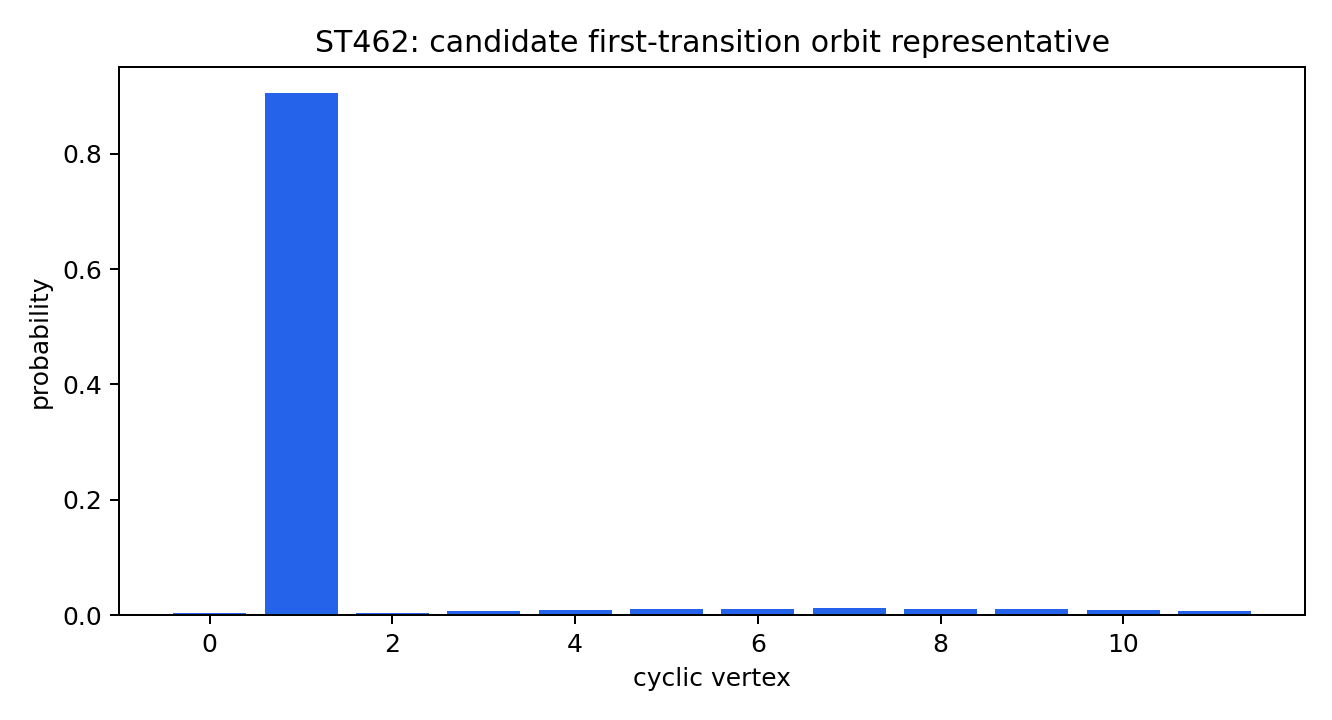
\includegraphics[width=.82\textwidth]{FIN_ST462_ST476_Figures/st462_transition_orbit.png}
\caption{Candidate first-transition representative. The plot is a numerical isolation result; its orbit size is later proved for the certified branch.}
\end{figure}

ST463 tested all 4,094 nontrivial uniform supports, refined 96 low-support faces and sampled 60,000 Dirichlet points. The best boundary refinement was $2.9771372811$ and the best unoptimized random value was $2.9463161100$, both above $R(p_*)$. This is adversarial evidence, not exhaustive proof.

ST469 gives an analytic boundary theorem.

\begin{theorem}[Boundary exclusion]
For every finite $g$, no boundary point of the simplex is a local or global minimizer of $V_g$.
\end{theorem}
\begin{proof}
If $p_j=0$, move to $p_\varepsilon=(1-\varepsilon)p+\varepsilon e_j$. The entropy change contains $\varepsilon\log\varepsilon$, which is negative and dominates every $O(\varepsilon)$ change of the bounded quadratic term as $\varepsilon\downarrow0$.
\end{proof}

The remaining competitor problem is therefore entirely interior.

\subsection{Autocatalytic feedback and the missing seed}

ST465 studied
\[
\dot g=\kappa(p-u)^TA(p-u)-\gamma g.
\]
At $(p,g)=(u,0)$ the right side is zero. A supplied perturbation generates a positive transient gain, but exact symmetry does not. This observation becomes a general theorem in Round IV.

\subsection{Dual dynamics}

For
\[
U_t=e^{-itA},\qquad P_t=e^{-tA},
\]
the modal response difference is
\[
h(x)=|e^{-ix}-e^{-x}|,qquad x=t\lambda.
\]
Its first positive global maximizer solves
\[
\sin x+\cos x=e^{-x},
\qquad x_*=2.284102297393826,
\]
and
\[
\boxed{h(x_*)=1.069432244918415.}
\]

\begin{figure}[H]\centering
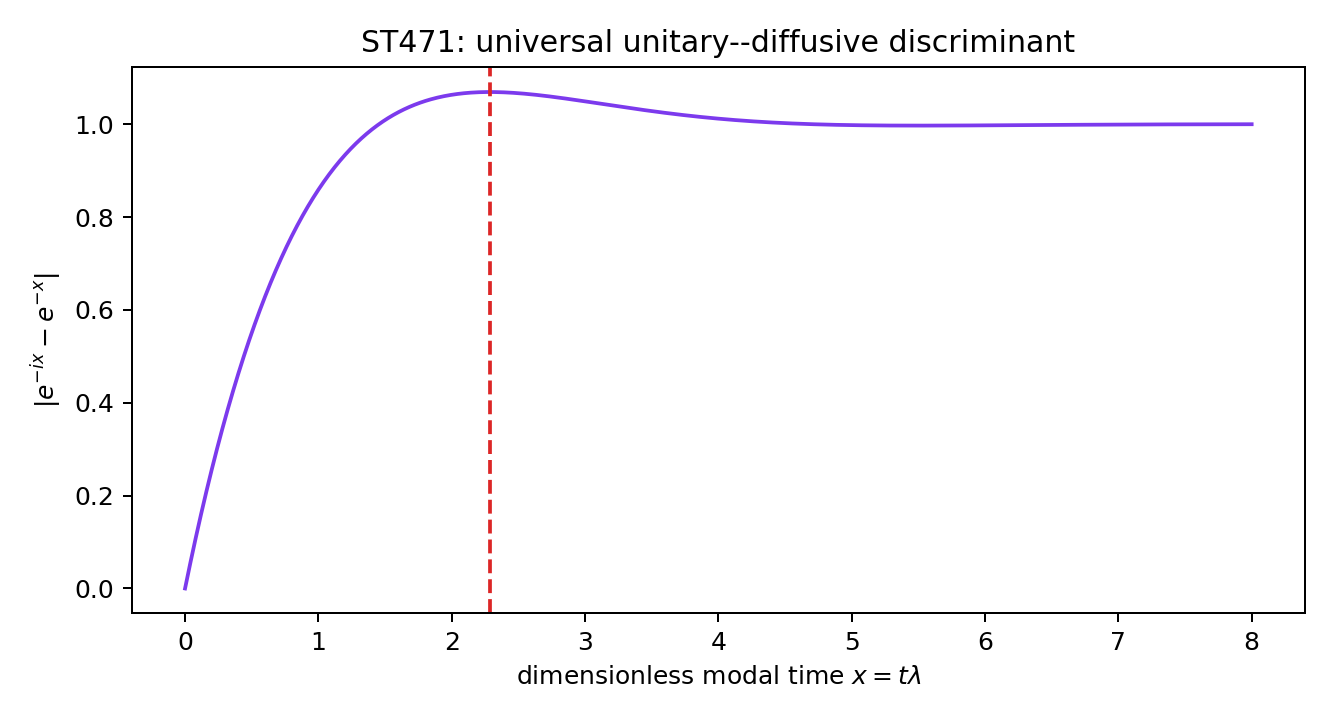
\includegraphics[width=.82\textwidth]{FIN_ST462_ST476_Figures/st471_dual_discriminant.png}
\caption{Universal dimensionless separation between coherent and diffusive scalar responses.}
\end{figure}

Approximate intertwining obeys simultaneous Duhamel bounds. If $\|\widetilde AR-RA\|\le\delta$ and $R$ is an isometry, then
\[
\|e^{-it\widetilde A}R-Re^{-itA}\|\le |t|\delta,
\qquad
\|e^{-t\widetilde A}R-Re^{-tA}\|\le t\delta.
\]
An isospectral conjugate fixing the constant mode changes fixed vertex heat and Born records by $0.02517$ and $0.04740$ in the declared fixture. Therefore eigenvalues alone are not the medium-independent information object.

\subsection{Round-I ledger}

\begin{longtable}{@{}p{.09\textwidth}p{.36\textwidth}p{.45\textwidth}@{}}\toprule
Program & Status & Result\\\midrule\endhead
ST462 & \strong & One twelve-member candidate orbit isolated at $2.9024964817477654$.\\
ST463 & \strong & No earlier competitor in declared boundary/random search.\\
ST464 & bounded stop & Old cover fails to certify $g=2.894$.\\
ST465 & \proven & Autocatalytic receiver requires a seed at $u$.\\
ST466 & exact sample & No support-4/5 circuit in 72,000 modular subsets.\\
ST467 & diagnostic & Stable floating degree-eight rank 1791.\\
ST468 & timeout & Singular returns no exact rank within 45 seconds.\\
ST469 & \proven & Boundary minimizers excluded for finite $g$.\\
ST470 & \proven & IR branch extended to $b=0.124$.\\
ST471 & \proven & Universal dual discriminant maximum.\\
ST472 & \proven & Linear intertwining stability for both channels.\\
ST473 & \proven & Spectrum-only information is insufficient.\\
ST474--476 & blocked & No strict gain, selector/scale source or evidence.\\\bottomrule
\end{longtable}

\section{Round II: ST477--ST491}

\subsection{Exact modular rank}

The degree-eight decomposable family contains 2,028 formal products. The complete degree-eight invariant space has Molien dimension 1,892. A new dependency-free C/OpenMP checker performed exact row elimination on the full $1892\times2028$ evaluation matrix:
\[
\rank_{\mathbb F_{1000003}}M
=\rank_{\mathbb F_{1000033}}M=1791.
\]
Thus each modular nullspace has dimension 237. Reduction modulo a prime cannot increase rational rank, while the Molien dimension gives an upper bound:
\begin{equation}\label{eq:rankbounds}
1791\le\rank_{\mathbb Q}M\le1892,
\qquad
136\le\dim\ker_{\mathbb Q}M\le237.
\end{equation}

\begin{figure}[H]\centering
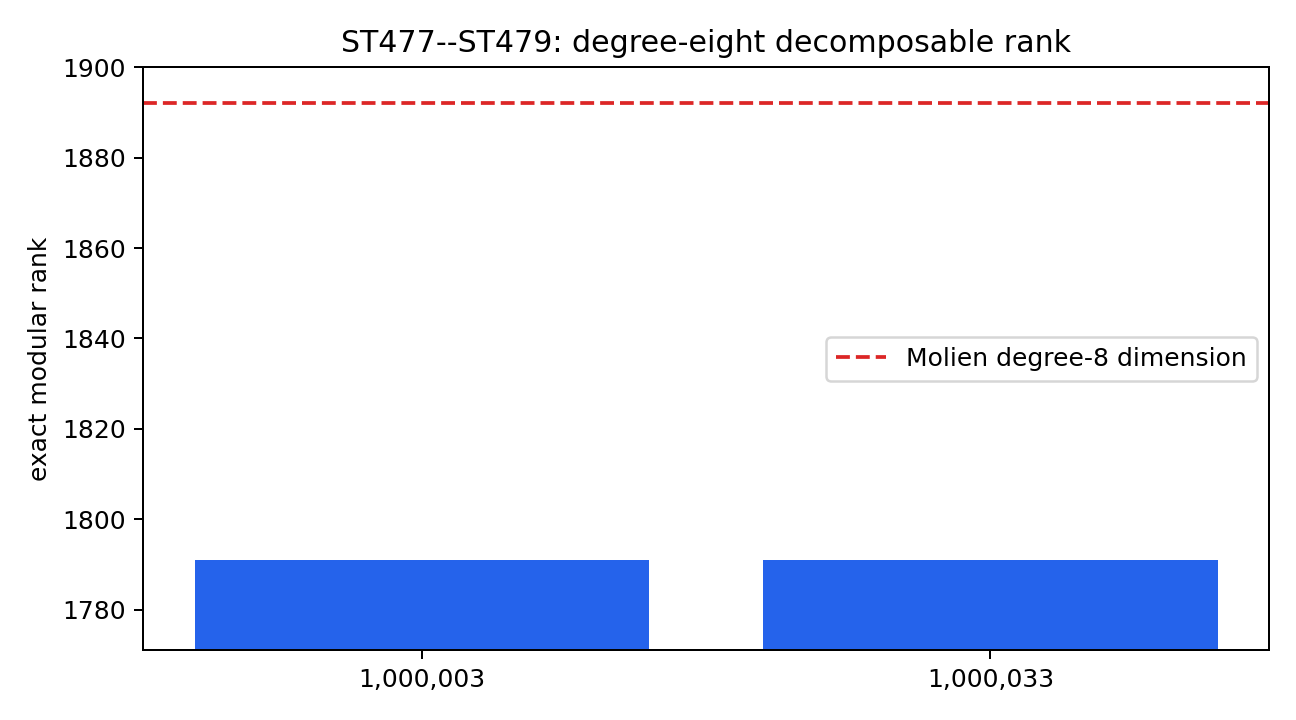
\includegraphics[width=.78\textwidth]{FIN_ST477_ST491_Figures/st477_modular_rank.png}
\caption{Exact finite-field ranks. The dashed Molien dimension is not silently replaced by the modular result.}
\end{figure}

\subsection{Orbit stabilizer theorem}

The interval-certified branch is parameterized by
\[
p=(p_0,p_1,p_2,p_3,p_4,p_5,p_6,p_5,p_4,p_3,p_2,p_1),
\]
with a unique dominant $p_0$ separated from all other coordinates by more than $0.893$.

\begin{theorem}[Branch stabilizer]
The stabilizer of every state in the certified crossing tube has order two, and its $D_{12}$ orbit has size twelve.
\end{theorem}
\begin{proof}
Reflection-even parameterization supplies one reflection. A unique dominant vertex excludes every nontrivial rotation. Two distinct reflections would compose to a nontrivial rotation. Hence the stabilizer contains exactly identity and one reflection, and orbit--stabilizer gives $24/2=12$.
\end{proof}

This proves the orbit size of the branch, not that the branch is globally first.

\subsection{Fluctuation source accounting}

For a zero-mean perturbation $\xi$ with covariance $\Sigma$,
\[
\mathbb E[\xi^TA\xi]=\Tr(A\Sigma).
\]
Consequently the stationary mean of the linear gain controller is
\[
\mathbb E g_\infty=\frac\kappa\gamma\Tr(A\Sigma).
\]
For tangent-isotropic $\Sigma=10^{-4}(I-\one\one^T/12)$, the exact response is $0.0019923687345$ and a 200,000-sample replay differs relatively by $6.79\times10^{-6}$.

\begin{figure}[H]\centering
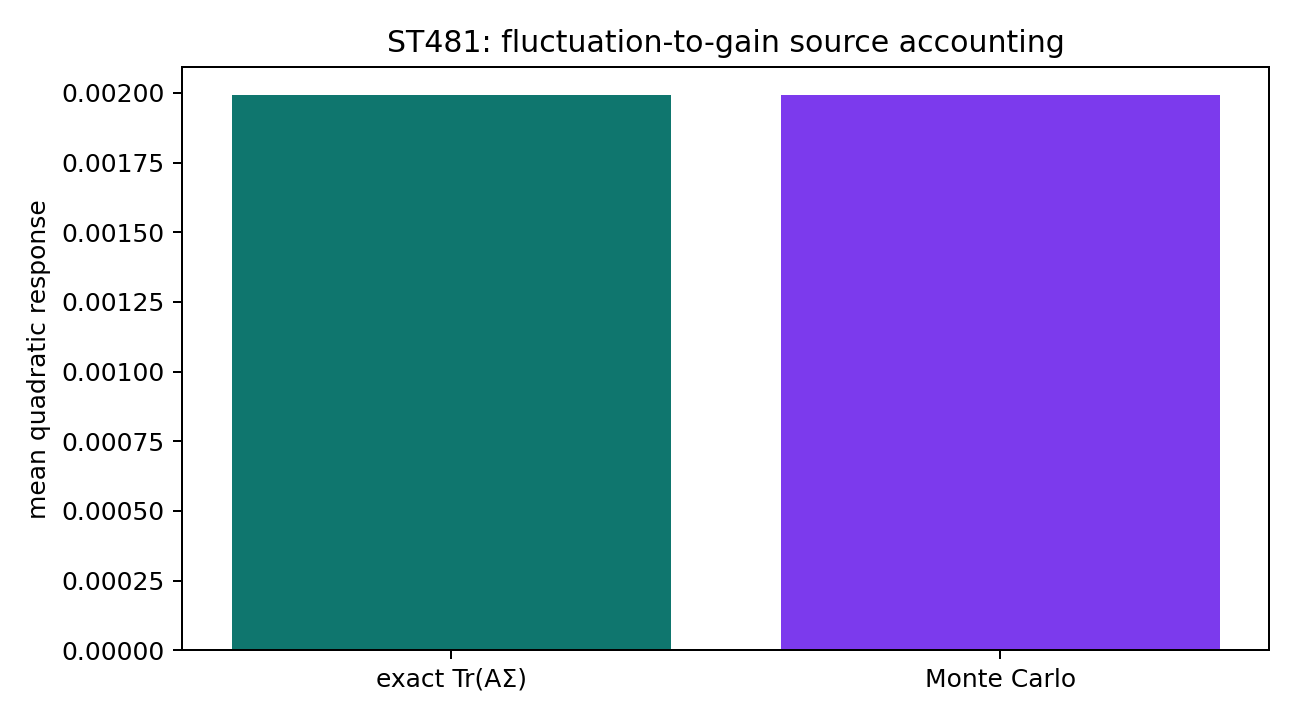
\includegraphics[width=.72\textwidth]{FIN_ST477_ST491_Figures/st481_fluctuation_gain.png}
\caption{The fluctuation identity works, but covariance is the new typed source resource.}
\end{figure}

Equivariant noise can realize a branch pathwise. Because the twelve branches form one transitive orbit and the noise law is invariant, every branch probability is $1/12$. Random realization is not canonical selection.

\subsection{Operational conjugacy}

If $B=QAQ^*$, then $f(B)=Qf(A)Q^*$ for every Borel $f$. Transporting states and effects,
\[
\rho'=Q\rho,\qquad M'=QM,
\]
preserves each matrix record. The numerical residual is below $1.3\times10^{-14}$. Fixed vertex labels without transported instruments are not equivalent. The medium-independent object is therefore an operational bundle, not a list of eigenvalues.

\subsection{Round-II ledger}
\begin{longtable}{@{}p{.09\textwidth}p{.36\textwidth}p{.45\textwidth}@{}}\toprule Program&Status&Result\\\midrule\endhead
ST477--478&\proven&Exact modular rank 1791 over two primes.\\
ST479&\proven&Characteristic-zero bounds \eqref{eq:rankbounds}.\\
ST480&\proven&Certified branch stabilizer order 2, orbit size 12.\\
ST481&\proven&Fluctuation covariance converts to mean gain.\\
ST482&\proven&Invariant noise realizes but does not select.\\
ST483&\proven&First modal unit-separation threshold $x=1.45367366646$.\\
ST484&\proven&Complete one-time operational conjugacy.\\
ST485&\proven&One raw unit cannot type both $\lambda$ and $\sqrt\lambda$ clocks.\\
ST486&\strong&ST342 branch and ST462 ratio candidate coincide numerically.\\
ST487&bounded stop&Unmodified cover fails at $g=2.8936$.\\
ST488&\proven&Repaired IR boxes extend to $b=0.196$.\\
ST489&exact sample&No support-6/8 circuit in 48,000 exact subsets.\\
ST490--491&blocked&No strict sources or independent evidence.\\\bottomrule\end{longtable}

\section{Round III: ST492--ST506}

\subsection{Three-prime and ensemble robustness}

Exact rank 1791 was reproduced over $p=1000003,1000033,1000037$ and on an independent integer point ensemble. All runs have the same ordered pivot fingerprint. Complete nullspace bases
\[
X_p\in\mathbb F_p^{2028\times237},\qquad M_pX_p=0,
\]
were generated for two primes and replayed on independent exact rows.

\begin{figure}[H]\centering
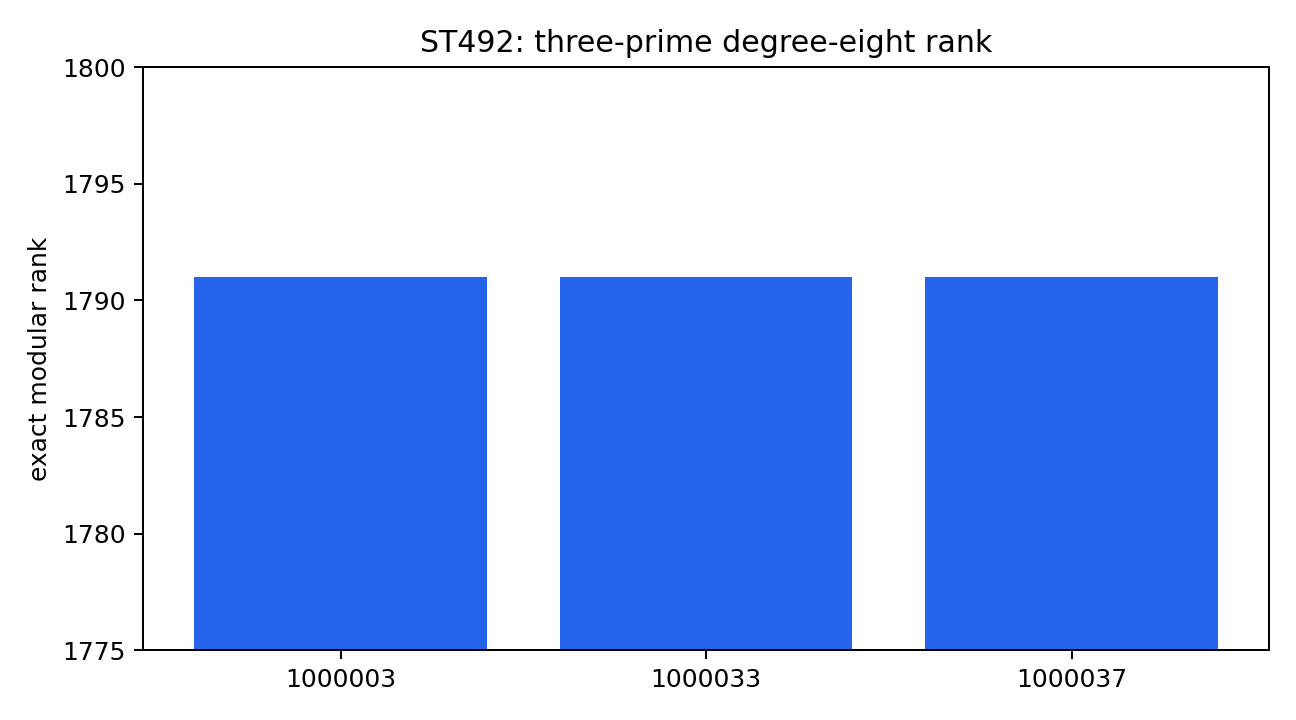
\includegraphics[width=.75\textwidth]{FIN_ST492_ST506_Figures/st492_three_prime_rank.png}
\caption{Three-prime exact rank agreement.}
\end{figure}

Two-prime rational reconstruction failed for all first eight aligned columns. The proper conclusion is not nonexistence: the selected modular basis has coefficient height exceeding the available rational-reconstruction window or is badly conditioned.

\subsection{Local transition curvature}

The reduced-logit Hessian of $R(p)$ at the candidate has minimum eigenvalue $0.00125490$ and Morse index zero. Across a further 160 BFGS/L-BFGS-B starts, all values return to the same candidate orbit. This is strong local evidence and stress testing, not a global certificate.

\begin{figure}[H]\centering
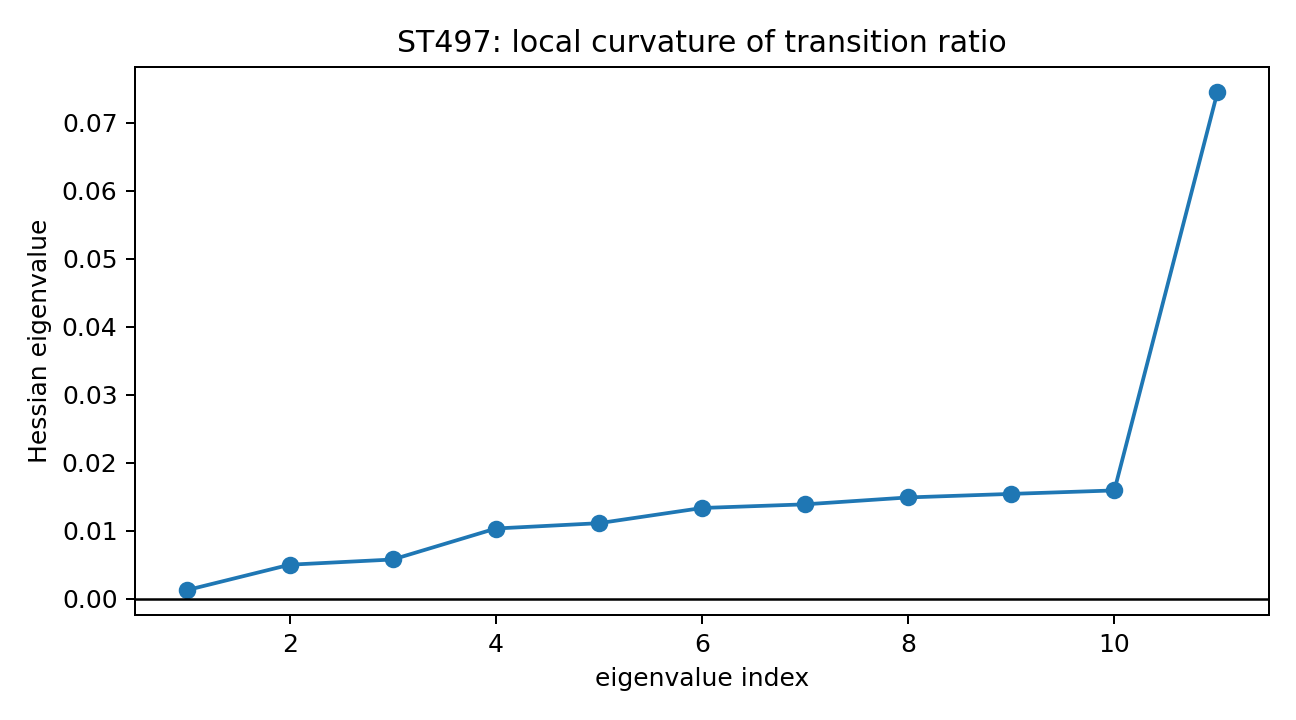
\includegraphics[width=.78\textwidth]{FIN_ST492_ST506_Figures/st497_transition_hessian.png}
\caption{Numerical reduced-logit Hessian of the transition ratio.}
\end{figure}

\subsection{Thermal and selector boundaries}

For a supplied thermal covariance on the mean-zero subspace,
\[
\Sigma=\theta A^+,
\qquad \Tr(A\Sigma)=11\theta,
\qquad \mathbb E g_\infty=11\frac\kappa\gamma\theta.
\]
This is an exact identity. Turning $\theta$ into $k_BT$ imports a bath, a temperature and energy calibration.

A biased branch law
\[
P_i(\varepsilon)=\frac{e^{\varepsilon b_i}}{\sum_j e^{\varepsilon b_j}}
\]
has
\[
P_i'(0)=\frac{b_i-\overline b}{12}.
\]
Nonuniform selection therefore requires a nonconstant bias vector, which is precisely an added selector source.

\subsection{Round-III ledger}
\begin{longtable}{@{}p{.09\textwidth}p{.36\textwidth}p{.45\textwidth}@{}}\toprule Program&Status&Result\\\midrule\endhead
ST492--494&\proven&Rank 1791 and pivot schema robust across primes/ensembles.\\
ST495&\proven&Two complete 237-vector modular nullspaces prepared.\\
ST496&bounded stop&Two-prime rational reconstruction fails for 8 probes.\\
ST497--498&\strong&Candidate is a strict local ratio minimum; 160 stress starts agree.\\
ST499&\proven&IR component continued to $b=0.2125$.\\
ST500&\proven&Thermal gain identity; dimensional bath remains external.\\
ST501&\proven&Bias is the selector source in the soft branch law.\\
ST502&\proven&One ideal modal response separates unitary and heat by one.\\
ST503&\proven&Operational conjugacy extends to finite multitime products.\\
ST504&\proven&Relative clock ratios obey perturbation bounds.\\
ST505--506&blocked&No strict source, $\mathbb Q$ closure or evidence.\\\bottomrule\end{longtable}

\section{Round IV: ST507--ST521}

\subsection{Five-prime nullspaces and failed high-modulus lift}

Three further modular bases were added, giving five primes, identical rank 1791, identical pivot schema, exact independent-row replay and a CRT modulus of 100 bits. Rational reconstruction still failed for all first sixteen aligned columns. This sharply changes the next algebraic task: adding a sixth similar prime without changing the basis is low value. One needs a height-reduced rational basis or a direct characteristic-zero syzygy construction.

\subsection{The symmetric-vacuum no-go theorem}

Let
\[
\Delta_{11}=\{p\in\R^{12}:p_i\ge0,\ \one^Tp=1\},
\quad u=\one/12,
\quad H_0=\{v:\one^Tv=0\}.
\]
The dihedral group acts transitively by coordinate permutations.

\begin{theorem}[Deterministic equivariant vacuum no-go]\label{thm:nogo}
Let $F:\Delta_{11}\to H_0$ be locally Lipschitz and $D_{12}$-equivariant. Then $F(u)=0$. The unique trajectory of $\dot p=F(p)$ with $p(0)=u$ is $p(t)=u$.
\end{theorem}
\begin{proof}
The point $u$ is fixed by every group element. Equivariance gives $gF(u)=F(gu)=F(u)$, so $F(u)$ lies in the fixed subspace of the permutation representation. Transitivity makes that fixed subspace $\operatorname{span}\{\one\}$. Tangency also gives $F(u)\in H_0$, and $H_0\cap\operatorname{span}\{\one\}=\{0\}$. Hence $F(u)=0$. Local uniqueness preserves the equilibrium.
\end{proof}

The theorem does not deny spontaneous symmetry breaking. It proves that a theory of such breaking must type the escape mechanism rather than claim that exact symmetric deterministic data silently choose a branch.

\begin{corollary}[Three-resource separation]
Pathwise departure, energetic amplification and canonical branch selection are distinct. They may be supplied respectively by a seed/noise realization, an active pump/covariance law and a noninvariant boundary/apparatus/bias.
\end{corollary}

\subsection{Wick continuation and the dephasing boundary}

In finite dimension $z\mapsto e^{-izA}$ is entire and
\[
\boxed{P_t=e^{-tA}=U_{-it}.}
\]
The matrix residual in the executed fixture is $5.69\times10^{-16}$. This is a mathematical analytic continuation, not a physical time process.

For the supplied dephasing generator
\[
\mathcal L_\gamma(\rho)=-i[A,\rho]-\gamma[A,[A,\rho]],
\]
the spectral entries evolve as
\[
\rho_{rs}(t)=e^{-it(\lambda_r-\lambda_s)}
e^{-\gamma t(\lambda_r-\lambda_s)^2}\rho_{rs}(0).
\]
Spectral populations are preserved, whereas $P_t$ transports classical vertex probability. Starting from the same vertex label in the declared embeddings gives $L^1$ record difference $0.6377202662$.

\begin{figure}[H]\centering
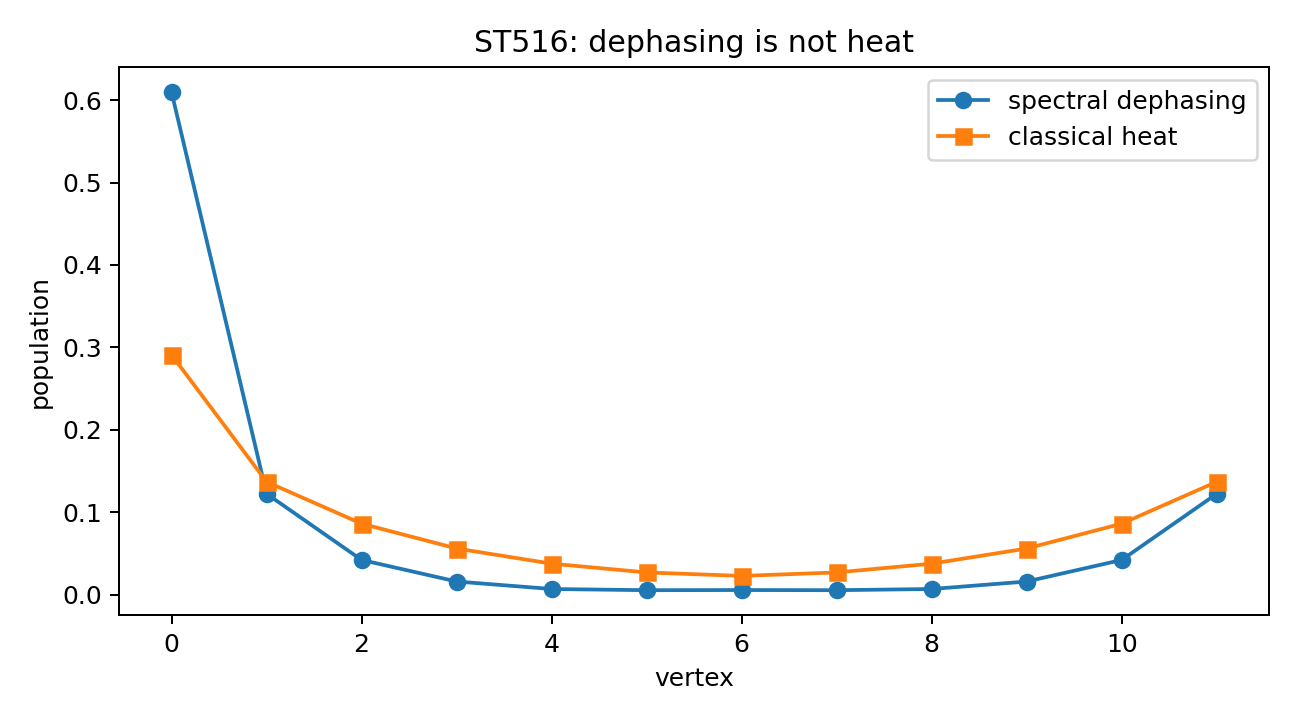
\includegraphics[width=.82\textwidth]{FIN_ST507_ST521_Figures/st516_dephasing_vs_heat.png}
\caption{Spectral dephasing and classical heat are different channels despite their common generator data.}
\end{figure}

\subsection{Certified branch curvature}

For a stationary state of \eqref{eq:Vg}, the simplex-tangent Hessian is
\[
H(p,g)=P\,[\operatorname{diag}(1/p)-gA]P,
\qquad P=I-\frac1{12}\one\one^T.
\]
At both endpoints of the certified crossing tube, the first tangent eigenvalue exceeds $5.61068$. Paying the root and gain interval perturbations leaves
\[
\boxed{\lambda_{\min}(H|_{H_0})>5.61067314.}
\]
Thus this branch is rigorously a strict local minimum throughout the tube. Global identity remains open.

\subsection{Round-IV ledger}
\begin{longtable}{@{}p{.09\textwidth}p{.36\textwidth}p{.45\textwidth}@{}}\toprule Program&Status&Result\\\midrule\endhead
ST507--508&\proven&Five aligned rank-1791 modular nullspace bases.\\
ST509--511&bounded stop&100-bit CRT reconstruction fails; exact $\mathbb Q$ obligations isolated.\\
ST512&\proven&Deterministic equivariant vacuum no-go.\\
ST513&\proven&Seed, gain and selector are distinct resources.\\
ST514&\proven&Finite Wick identity $P_t=U_{-it}$, not operational equivalence.\\
ST515&\proven&Exact spectral dephasing formula.\\
ST516&\proven&Dephasing is not classical heat.\\
ST517&\conditional&Dual-response separation survives error $\varepsilon<1/2$.\\
ST518&\proven&IR component continued to $b=0.2345$.\\
ST519&\proven&Positive paid curvature on crossing tube.\\
ST520--521&blocked&No strict sources, $\mathbb Q$ closure or evidence.\\\bottomrule\end{longtable}

\section{Round V: ST522--ST536}

\subsection{Conditioned basis and algebraic stop}

Pivoted QR separates 1,791 columns with smallest accepted diagonal $1.95\times10^{-5}$ from a first rejected diagonal $1.74\times10^{-15}$. Reordering columns accordingly is admitted exactly over all five primes, and the resulting modular nullspaces replay exactly on unseen rows. Nevertheless, rational reconstruction fails for all 32 probed conditioned columns. Therefore the obstruction is not cured by elementary numerical conditioning.

The accepted statement remains \eqref{eq:rankbounds}. A proof of $\rank_{\mathbb Q}=1791$ must provide one of:
\begin{enumerate}
\item all 237 rational relations with exact polynomial verification modulo $x_0+\cdots+x_{11}$;
\item an independent characteristic-zero upper-rank theorem;
\item a structure-aware elimination producing the same kernel dimension.
\end{enumerate}

\subsection{Necessity of the no-go hypotheses}

Each hypothesis of Theorem~\ref{thm:nogo} has a removal witness.

\begin{table}[H]\centering\caption{Axiom-removal audit.}
\begin{tabularx}{\textwidth}{@{}p{.26\textwidth}X@{}}\toprule Removed premise&Escape mechanism\\\midrule
Equivariance&A constant tangent bias moves $u$.\\
Exact uniform initial state&An arbitrarily small nonuniform seed may evolve.\\
Determinism/local uniqueness&A set-valued or nonunique flow may choose branches.\\
Transitivity/zero fixed tangent space&A nontransitive action may have a nonzero fixed tangent direction.\\
Tangency&Normal motion may leave the probability simplex.\\\bottomrule
\end{tabularx}\end{table}

For an analytic invariant gain controller
\[
\dot g=F(g,I_1(p),\ldots,I_m(p)),\qquad I_j(u)=0,
\]
one has
\[
\dot g(0)=F(0,0,\ldots,0).
\]
A nonzero first gain derivative therefore requires a constant/source term or an invariant with a supplied nonzero vacuum value. This is the minimal source obligation.

On a transitive twelve-branch orbit, an invariant deterministic selector is impossible and an invariant stochastic selector is uniform. A nonuniform or deterministic selection factors through a symmetry-breaking datum. For scale, a scale-invariant strict datum cannot select a point of a free positive calibration torsor; one must provide a scale-charged $S_+$ or explicit conversion axioms.

\subsection{Three-channel separation}

The common spectrum supports three generically distinct responses:
\[
e^{-it\lambda},\qquad e^{-t\lambda},\qquad
e^{-it\lambda-\gamma t\lambda^2}.
\]
For the largest strict eigenvalue at $t=0.8$, $\gamma=0.4$, their pairwise distances are
\[
d_{U,H}=1.05603,
\qquad d_{U,D}=0.82717,
\qquad d_{H,D}=0.26321.
\]

\begin{figure}[H]\centering
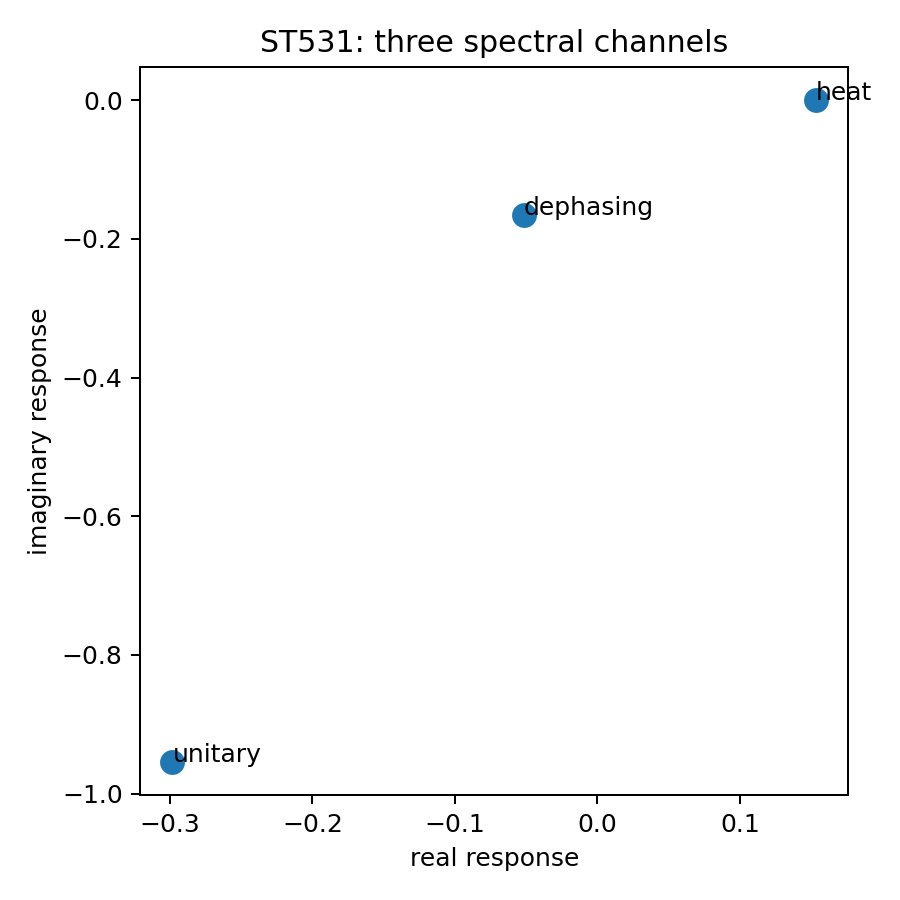
\includegraphics[width=.68\textwidth]{FIN_ST522_ST536_Figures/st531_three_channels.png}
\caption{Three spectral responses of one mode. Common spectral origin does not collapse channel semantics.}
\end{figure}

After paying response error $0.05$ for each model, the minimum pairwise separation remains $0.16321$. This is an ideal linear tester bound. It lacks a finite-shot likelihood, detector and laboratory record.

\subsection{Final transition and IR status}

The consolidated transition evidence is:
\begin{itemize}
\item global theorem: $g_*\in[2.8934,2.9024964917477667]$;
\item candidate: $2.9024964817477654$;
\item 268 multistart hits across declared algorithms;
\item exact branch orbit size 12;
\item boundary minimizers excluded;
\item paid local curvature $>5.61067314$;
\item missing step: exclude all other interior orbits below the candidate.
\end{itemize}

Adaptive interval continuation reaches $b=0.2435$. Increasing radius factors to 32 does not certify the next template to $0.3$. This is a new method stop, not a detected fold.

\begin{figure}[H]\centering
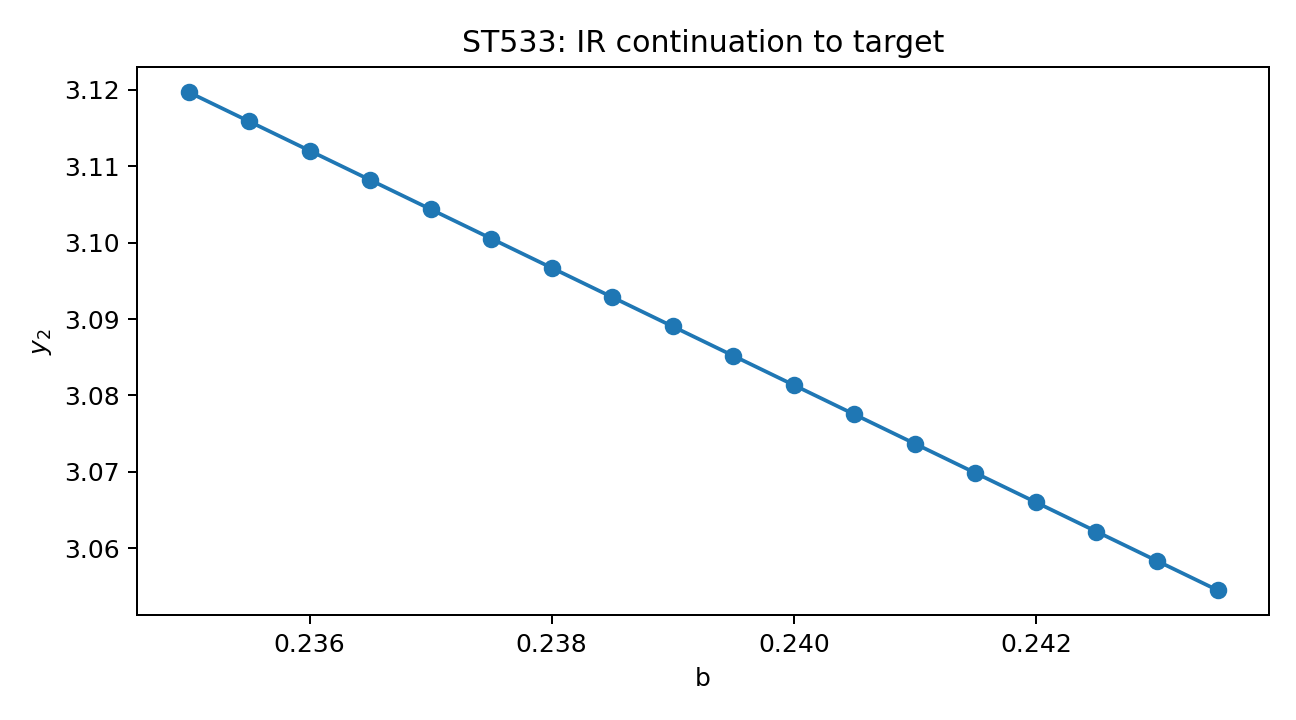
\includegraphics[width=.82\textwidth]{FIN_ST522_ST536_Figures/st533_ir_target.png}
\caption{Fifth-round continuation of the same local IR component until the new template stop.}
\end{figure}

\subsection{Round-V ledger}
\begin{longtable}{@{}p{.09\textwidth}p{.36\textwidth}p{.45\textwidth}@{}}\toprule Program&Status&Result\\\midrule\endhead
ST522&diagnostic&QR-conditioned order has floating rank 1791.\\
ST523&\proven&Conditioned order admitted over five exact fields.\\
ST524--526&bounded stop&Conditioned rational lift fails; $\mathbb Q$ rank remains open.\\
ST527&\proven&All no-go premises have explicit removal witnesses.\\
ST528&\proven&Invariant gain needs a nonzero vacuum/source term.\\
ST529&\proven&Invariant selector is impossible or randomized uniformly.\\
ST530&\proven&Strict scale source or conversion-axiom dichotomy.\\
ST531&\proven&Three spectral channels are pairwise distinct.\\
ST532&\conditional&Ideal three-model tester retains positive margin.\\
ST533&\proven&IR continuation reaches $b=0.2435$ and stops.\\
ST534&consolidated&Candidate first orbit is strong, global identity open.\\
ST535--536&blocked&No strict closure or independent evidence.\\\bottomrule\end{longtable}

\section{Round VI: ST537--ST551}

\subsection{Where the 237 degree-eight relations actually enter}

Round VI replaces the undifferentiated 2,028-column problem by four declared families:
\[
q^4\ (126),\qquad q^2p_4\ (672),\qquad p_4p_4\ (528),\qquad qp_6\ (702).
\]
Exact elimination over both $\mathbb F_{1000003}$ and $\mathbb F_{1000033}$ gives
\[
\begin{array}{c|cccc}
\text{family}&q^4&q^2p_4&p_4p_4&qp_6\\\hline
\text{columns}&126&672&528&702\\
\text{rank}&126&672&528&702.
\end{array}
\]

\begin{theorem}[Separate characteristic-zero independence]
Each of the four declared degree-eight families is linearly independent over $\mathbb Q$.
\end{theorem}
\begin{proof}
Every column has integer coefficients. A rational dependence can be cleared to a primitive integer dependence. Reduction modulo a prime cannot have full column rank if such a dependence exists. Each displayed modular block has rank equal to its column count, so no rational dependence exists inside any single family.
\end{proof}

The cumulative ranks are more informative:
\[
126,\qquad798,\qquad1288,\qquad1791.
\]
Thus the first two families remain jointly independent. Adding $p_4p_4$ contributes only 490 new directions and creates exactly 38 modular cross-family relations. Adding $qp_6$ contributes 503 new directions and creates another 199, totaling 237.

\begin{figure}[H]\centering
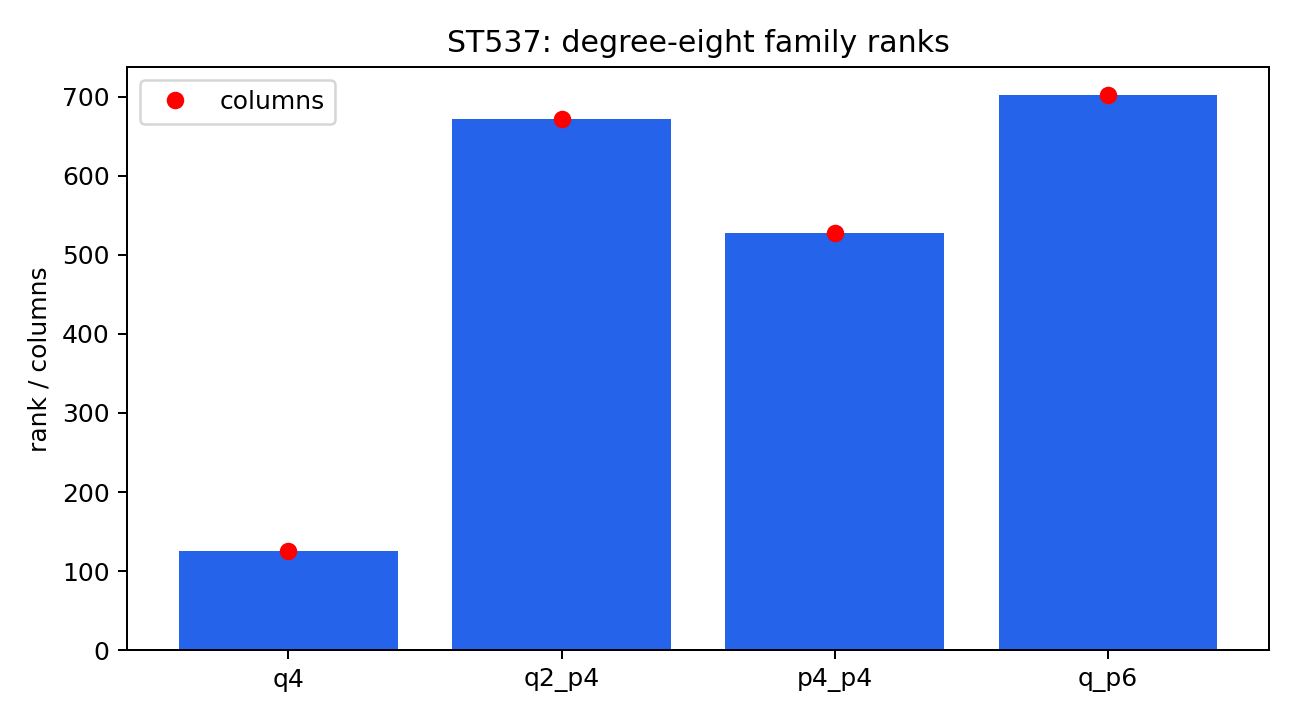
\includegraphics[width=.82\textwidth]{FIN_ST537_ST551_Figures/st537_family_ranks.png}
\caption{Every family is individually full rank; dependencies arise only in their intersections.}
\end{figure}

This is a genuine structural improvement. Future rational reconstruction should first attack the 38-relation interface among $q^4$, $q^2p_4$ and $p_4p_4$, then the 199-relation extension introduced by $qp_6$. It should not treat the full kernel as an unstructured 237-dimensional object.

\subsection{Transition subfamilies and the remaining global gap}

All 2,047 two-level subset patterns, modulo complements, were optimized. Their best ratio is
\[
R_{\rm two-level}=2.9125665644276797,
\]
which exceeds the candidate by
\[
R_{\rm two-level}-R(p_*)=0.0100700826799143.
\]
No two-level state beats the candidate. The scalar minimizations are high-accuracy numerical and are not promoted to interval theorems.

Within the full reflection-even six-dimensional quotient, 240 starts again find the candidate value $2.902496481747765$ and no lower value. Forty-six stationary-value clusters appear, so the search is not trivial; only 24 starts reach the best orbit. Combined with the paid local curvature, this is strong evidence but not a compact quotient cover.

The first-transition obligation is now sharply localized:
\[
\boxed{\text{exclude every other interior, genuinely multilevel orbit for }
g\in[2.8934,2.9024964817477654).}
\]

\subsection{Symmetric stochastic realizations and nonunique flows}

In a 240,000-sample isotropic tangent-Gaussian replay, a covariant nearest-orbit rule gives all twelve branch frequencies within $6.59\times10^{-4}$ of $1/12$; the Pearson statistic is $6.1591$ with 11 degrees of freedom.

\begin{figure}[H]\centering
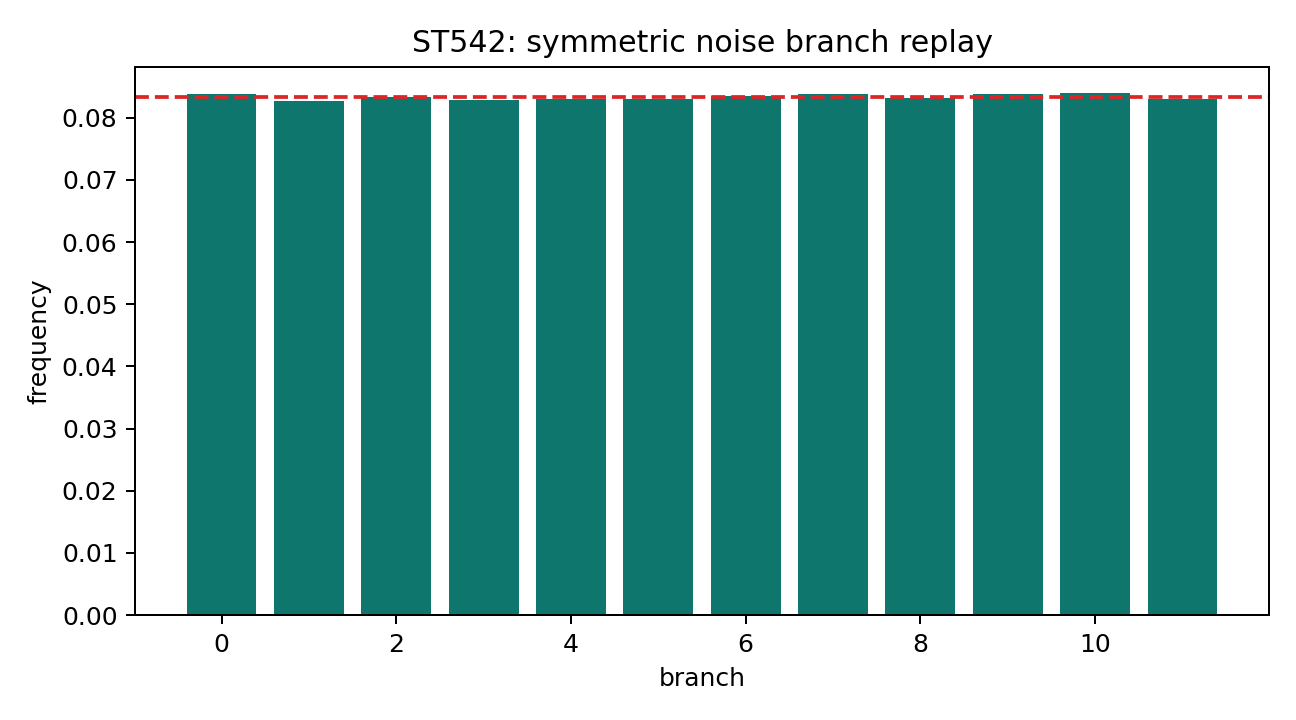
\includegraphics[width=.82\textwidth]{FIN_ST537_ST551_Figures/st542_branch_frequencies.png}
\caption{Symmetric noise realizes branches with the uniform law; it does not prefer a canonical member.}
\end{figure}

Dropping uniqueness evades Theorem~\ref{thm:nogo}. The scalar differential inclusion
\[
\dot z\in\operatorname{Sign}(z),\qquad z(0)=0,
\]
admits $z=0$, $z=t$, $z=-t$ and delayed departures. Yet the branch choice is now carried by the solution-selection rule or stochastic regularization. Nonuniqueness relocates the selector rather than deriving it.

For an irreducible $D_{12}$-covariant Markov generator on the twelve branches, the uniform law is stationary and unique. A symmetric Markov ``selector'' therefore randomizes uniformly. Nonuniform stationary choice requires broken covariance or reducibility together with initial-sector information.

\subsection{Finite-shot and completely positive operational tests}

For the supplied isotropic two-quadrature Gaussian response model with $\sigma=0.05$, the minimum pairwise three-channel Chernoff exponent is
\[
C_{\min}=3.4640101962673517.
\]
A three-pair union bound at target error $0.01$ requires only two independent response samples in this idealized fixture. This is a conditional synthetic sample bound, not detector performance.

Operational conjugacy was also replayed for a completely positive three-Kraus fixture, giving record residual $1.80\times10^{-16}$. The fixture was not claimed trace preserving; a physical process tensor still needs normalized instruments and event registers.

Joint ideal channel observations
\[
(y_U,y_H,y_W)=(a\lambda,b\lambda,c\sqrt\lambda)
\]
remain invariant under
\[
\lambda\mapsto q\lambda,qquad(a,b,c)\mapsto(a/q,b/q,c/\sqrt q).
\]
They identify calibration ratios but leave one positive common scaling orbit. Even all three channels do not generate absolute seconds.

\subsection{IR and operational package status}

Using the inherited certified endpoint rather than the remote original seed, an ultra-fine chart extends the same local IR component to
\[
\boxed{b=0.2530000000}.
\]
The minimum inclusion margin is $1.09\times10^{-7}$ and maximum weighted contraction $0.01944$. Radius factors as high as 64 are then insufficient. A separate 13-point grid with 80 starts per point from $b=0.24$ to $0.3$ finds exactly one positive root cluster at every point. This is numerical complement evidence, not a global interval degree theorem.

The minimal conditional physical architecture remains
\[
W_0+\mathrm{CA}+\mathrm{SA}+\mathrm{OA}.
\]
Removing CA leaves absolute dimensions unidentified; removing SA leaves oriented branch claims unidentified; removing OA leaves no state-to-record map. The packages close different obligations and cannot be substituted for one another.

\subsection{Round-VI ledger}
\begin{longtable}{@{}p{.09\textwidth}p{.36\textwidth}p{.45\textwidth}@{}}\toprule Program&Status&Result\\\midrule\endhead
ST537&\proven&Exact blockwise modular ranks; every family is full column rank.\\
ST538&\proven&Cumulative ranks $126,798,1288,1791$ localize 38+199 relations.\\
ST539&\proven&All four families separately independent over $\mathbb Q$.\\
ST540&strong/exhaustive class&All two-level patterns tested; none beats the candidate.\\
ST541&\strong&Reflection quotient: 240 starts, no lower orbit.\\
ST542&\strong&Symmetric-noise frequencies agree with $1/12$.\\
ST543&\proven&Nonunique flow evades vacuum no-go but relocates selector.\\
ST544&\conditional&Gaussian finite-shot bound gives $n=2$ in supplied fixture.\\
ST545&\proven&Completely positive operational-conjugacy record invariance.\\
ST546&\proven&Joint calibration leaves one positive torsor.\\
ST547&\proven&Fine-chart local IR extension reaches $b=0.253$.\\
ST548&\strong&One numerical positive-root cluster across $b\in[0.24,0.3]$.\\
ST549&blocked&No new strict source provider.\\
ST550&\proven&CA, SA and OA have distinct minimal roles.\\
ST551&blocked&No independent empirical evidence.\\\bottomrule\end{longtable}

\section{Falsification ledger and failed methods}

\begin{longtable}{@{}p{.28\textwidth}p{.28\textwidth}p{.35\textwidth}@{}}\caption{Methods that failed and what the failure means.}\\\toprule Attempt&Observed failure&Licensed conclusion\\\midrule\endfirsthead\toprule Attempt&Observed failure&Licensed conclusion\\\midrule\endhead
Unmodified global $(t,\rho)$ cover above 2.8934&Failed leaves at paid numerical floor after 666,920 accepted leaves&Architecture stop; not a competitor and not failure of the global claim.\\
Singular full rank&45-second timeout&Implementation/resource stop only.\\
Sequential five-prime CRT basis&0/16 rational probe columns reconstructed&Naive basis has excessive height; no rational no-go.\\
QR-conditioned five-prime basis&0/32 reconstructed&Elementary conditioning is insufficient; exact $\mathbb Q$ rank remains open.\\
Random support 4--8 circuit scans&No circuits in declared exact samples&Reproducible evidence for dense relations, not an exhaustive support theorem.\\
IR radius enlargement&Successive inherited charts stop at $b=0.253$ despite factor 64&Certificate-template stop; no fold or physical cutoff proved.\\
Symmetric deterministic feedback&Cannot move exact $u$&Theorem-grade class no-go; a typed escape resource is necessary.\\
Symmetric noise as selector&Uniform branch law&Random realization is not canonical selection.\\\bottomrule\end{longtable}

\section{Deepest interpretation after six rounds}

The six rounds reinforce the central FIN interpretation rather than replace it. The strict object is a finite, dimensionless spectral-information generator. Its one spectral measure produces coherent, diffusive, wave, resolvent and response calculi. Context and instruments determine which shadow is observed.

The new structural conclusion is sharper:
\[
\boxed{\text{symmetry supplies a space of possibilities, not the event selecting one possibility}.}
\]
An exactly symmetric deterministic strict core cannot initiate the event. A physical completion needs an explicit law for fluctuation/initial condition, energy or informational pump, selector/apparatus frame and dimensional calibration. These may ultimately be derived from a richer nadsoliton object, but they are not functions of the present radial spectrum.

This is a scientifically useful breakthrough because it converts a vague ``missing selector'' into an axiom-ranked obstruction. It also prevents an incorrect identification of noise, gain and measurement. It is not a Theory-of-Everything closure.

\section{Recommended next research cycle: ST552--ST566}

The next cycle should exploit the newly localized $38+199$ cross-family structure. It should not return to an undifferentiated 2,028-column lift.

\begin{longtable}{@{}p{.08\textwidth}p{.29\textwidth}p{.52\textwidth}@{}}\caption{Ranked next studies.}\\\toprule Rank&Programme&Acceptance criterion / falsifier\\\midrule\endfirsthead\toprule Rank&Programme&Acceptance criterion / falsifier\\\midrule\endhead
1&ST552 stage-one conditioned pivot design&Construct a height-reduced basis for the first 1,326 columns and its 38-dimensional cross-family kernel.\\
2&ST553 five-prime stage-one nullspaces&Require exact rank 1,288, common free schema and unseen-row replay.\\
3&ST554 stage-one rational reconstruction&Lift all 38 aligned vectors; failure must report a coefficient-height bound rather than nonexistence.\\
4&ST555 exact polynomial verification&Check divisibility by $x_0+\cdots+x_{11}$ for every lifted relation. No sampled evaluation is sufficient.\\
5&ST556 stage-one characteristic-zero rank&Promote rank 1,288 only after both an exact lower minor and 38 exact relations.\\
6&ST557 two-level interval certificate&Replace the numerical scalar minimizations by outward one-dimensional enclosures for all subset orbits.\\
7&ST558 reflection quotient cover&Cover the six-dimensional reflection-even quotient or issue a finite resource-bounded stop.\\
8&ST559 global interior transition cover&Use boundary and two-level exclusion to attack only genuinely multilevel interior states.\\
9&ST560 equivariant Markov selector theorem&Formalize when uniform branch randomization is unique and which premise permits nonuniform selection.\\
10&ST561 finite-shot replay&Freeze a synthetic event likelihood and compare its empirical error with the analytic Chernoff bound.\\
11&ST562 CPTP operational conjugacy&Use a trace-preserving instrument and classical register, not only a CP fixture.\\
12&ST563 minimal calibration anchor&Prove the one-anchor statement inside the admitted channel-specific scale model without confusing it with full CA.\\
13&ST564 analytic IR reparameterization&Replace further radius inflation at $b=0.253$ by a new chart; repeated finer boxes are now gated.\\
14&ST565 strict admission gate&Open only for a genuinely new seed, gain, selector or scale provider.\\
15&ST566 evidence gate&Accept only independently custodied event records; local synthetic output remains nonempirical.\\\bottomrule\end{longtable}

\section{Final conclusions}

\begin{enumerate}
\item The first-transition candidate is now exceptionally well characterized: interior, reflection-even, orbit size twelve, strict local curvature, and 268 multistart hits. Its global-first identity is still open.
\item The degree-eight decomposable family has exact modular rank 1791 and nullity 237 over five primes and robust point ensembles. Every generating family is separately independent over $\mathbb Q$; the 237 relations are localized as 38 plus 199 cross-family relations. Full characteristic-zero equality is not proved.
\item The exact uniform state cannot spontaneously leave under deterministic, locally unique, $D_{12}$-equivariant tangent dynamics. This is the principal new no-go theorem.
\item Fluctuation, gain and selection are distinct. Covariance can source mean quadratic gain; invariant noise produces uniform branch probabilities; a nonuniform selector requires an asymmetric datum.
\item The dual dynamics remains central. Unitary and heat channels are analytically related by imaginary time but operationally different. Dephasing is a third, distinct spectral channel.
\item Operationally medium-independent information requires projectors/generator together with transported preparations, interventions, effects and records. Spectrum alone is incomplete.
\item The local IR branch is certified through $b=0.253$; no physical length or continuum limit follows.
\item No strict active source, nonpremise selector, absolute unit, laboratory evidence, legacy-to-strict completion, role transfer, Standard Model, gravity, $L_{\rm total}$ or ToE closure is obtained.
\end{enumerate}

\claimbox{\textbf{Six-round verdict.} FIN now contains a theorem-level explanation of why exact symmetric strict data cannot by themselves produce the first realized asymmetric world in the deterministic class, together with a blockwise localization of the degree-eight algebraic obstruction. The missing physical principle must supply an escape resource, a sustaining gain law, a selector and calibration/operations, or prove how a richer nadsoliton object generates them. This is a major clarification of the theory's architecture, not empirical confirmation.}

\appendix
\section{Artifact inventory}

The principal machine-readable outputs are:
\begin{itemize}
\item \texttt{FIN\_ST462\_ST476\_Results.json} and 15 program packets;
\item \texttt{FIN\_ST477\_ST491\_Results.json} and exact modular rank packets;
\item \texttt{FIN\_ST492\_ST506\_Results.json}, \texttt{FIN\_ST495\_Degree8\_Modular\_Nullspaces.npz};
\item \texttt{FIN\_ST507\_ST521\_Results.json}, \texttt{FIN\_ST507\_FivePrime\_Degree8\_Modular\_Nullspaces.npz};
\item \texttt{FIN\_ST522\_ST536\_Results.json}, \texttt{FIN\_ST523\_QR\_Conditioned\_FivePrime\_Nullspaces.npz};
\item \texttt{FIN\_ST537\_ST551\_Results.json} and its blockwise-rank, transition, stochastic, operational and IR packets;
\item six Python research scripts, the exact C modular-rank checker and six unit-test modules;
\item figure directories for each round.
\end{itemize}

\section{Reproducibility and nonclaims}

The authoritative rerun sequence is
\begin{verbatim}
python3 fin_st462_st476_research.py
python3 fin_st477_st491_research.py
python3 fin_st492_st506_research.py
python3 fin_st507_st521_research.py
python3 fin_st522_st536_research.py
python3 fin_st537_st551_research.py
python3 -m unittest -v test_fin_st462_st476.py \
  test_fin_st477_st491.py test_fin_st492_st506.py \
  test_fin_st507_st521.py test_fin_st522_st536.py \
  test_fin_st537_st551.py
\end{verbatim}

The report makes no network-dependent literature claim and includes no external data. It does not discharge $QW\text{-}2191$, identify a physical vacuum, derive a unit-bearing action, or validate an apparatus. All future research PDFs remain English.

\end{document}
